\documentclass[11pt]{article}

% PACKAGES!
\usepackage{amsmath,amsfonts,amssymb}
\usepackage{graphicx,epsfig,xcolor,epstopdf}
\usepackage{enumerate}
%\usepackage{algorithm}
%\usepackage{algorithmic}
\usepackage{lscape}
\usepackage{multirow, multicol}
\PassOptionsToPackage{hyphens}{url}
\usepackage[unicode=true,pdfusetitle,
 bookmarks=true,bookmarksnumbered=true,bookmarksopen=false,
 breaklinks=false,pdfborder={0 0 1},backref=false,colorlinks=false]{hyperref}
\usepackage{booktabs,dsfont,rotating,pdflscape}
\usepackage[small,bf]{caption} % custom caption style: small and bold
\usepackage{subcaption}
\usepackage{courier}
\usepackage{soul}
\setcounter{MaxMatrixCols}{20}% allow up to 20-column matrices
\usepackage[margin=1.00in, paperwidth=8.5in, paperheight=11in]{geometry}
\usepackage[square,authoryear]{natbib}
\usepackage[nottoc]{tocbibind}
\usepackage[linesnumbered,lined,boxed,commentsnumbered]{algorithm2e}

% NEW COMMANDS
\renewcommand\contentsname{TABLE OF CONTENTS}
\renewcommand{\tocbibname}{References}

\begin{document}

%%%%%%%%%%%%%%%%%%%%%%%%%%%%%%%%%%%%%%%%%%%%%%%%%%%
% TITLE PAGE
%%%%%%%%%%%%%%%%%%%%%%%%%%%%%%%%%%%%%%%%%%%%%%%%%%%

\begin{titlepage} 

\centering
	{\huge\bfseries TreeScaper CLV Manual \par}
	\vspace{1cm}
	{\LARGE\bfseries Beta Version\par}
	\vspace{1cm}
	{\Large\bfseries \today\par}
	\vspace{1.5cm}
	{\Large Jeremy Ash$^{2,4}$, \\ Jeremy M. Brown$^{2}$, \\ David Morris$^{2}$, \\ Guifang Zhou$^{2}$, \\ Wen Huang$^{1}$, \\ Melissa Marchand$^{3}$, \\ Paul Van Dooren$^{1}$, \\ Kyle A. Gallivan$^{3}$, \\ and Jim Wilgenbusch$^{5}$\par}
	\vspace{3.5cm}
	{\small $^{1}$Department of Mathematical Engineering, ICTEAM, \\ Universit\'{e} catholique de Louvain, Belgium, \\ wen.huang@uclouvain.be \par}
	\vspace{0.5cm}
	{\small $^{2}$ Department of Biological Sciences and Museum of Natural Science, \\ Louisiana State University, Baton Rouge, LA, USA \par}
	\vspace{0.5cm}
	{\small $^{3}$ Department of Mathematics, \\ Florida State University, Tallahassee, FL, USA \par}
	\vspace{0.5cm}
	{\small $^{4}$ Current Address: Bioinformatics Research Center, \\ North Carolina State University, Raleigh, NC, USA \par}
	\vspace{0.5cm}
	{\small $^{5}$ Minnesota Supercomputing Institute, \\ University of Minnesota, Minneapolis, MN, USA \par}
	\vfill


% Bottom of the page
	

\end{titlepage}

\begin{center}\tableofcontents\end{center}
%\listoffigures
\newpage

%%%%%%%%%%%%%%%%%%%%%%%%%%%%%%%%%%%%%%%%%%%%%%%%%%%
% INTRODUCTION
%%%%%%%%%%%%%%%%%%%%%%%%%%%%%%%%%%%%%%%%%%%%%%%%%%%
\section{INTRODUCTION}\label{sect:Introduction}

Phylogenetic trees are now routinely inferred from enormous genome-scale data sets, revealing extensive variation in phylogenetic signal both within and between individual genes. This variation may result from a wide range of biological phenomena, such as recombination, horizontal gene transfer, or hybridization.  It may also indicate stochastic and/or systematic error.  However, current approaches for summarizing the variation in a tree set typically condense it into point estimates, such as consensus trees, resulting in extensive loss of information. \\


We have written TreeScaper to provide a set of visual and quantitative tools for exploring and characterizing the full complement of phylogenetic information contained in a tree set. These tools can be broadly categorized into three types: (1) utilities for calculating basic information about topologies and bipartitions, (2) visualization of treespace in $2-$ or $3-$dimensional space through non-linear dimensionality reduction (NLDR), and (3) detection and delineation of distinct communities of trees. \\


{\it Tree objects} -- Much of TreeScaper's functionality requires calculating distances between trees, transforming distances into affinities, translating trees into their component bipartitions, and summarizing how these bipartitions are distributed across trees (i.e., their variances and covariances). However, this information can also be useful in its own right. Therefore, TreeScaper provides a set of built-in utilities to calculate a range of useful tree- and bipartition-related summaries. Once calculated, these values may be used for other tasks in TreeScaper or may be written to file for use in other applications. \\



{\it NLDR} -- One way to visually explore tree sets is to plot a $2-$ or $3-$dimensional representation of treespace using non-linear dimensionality reduction (NLDR; Fig.~\ref{fig1}). This approach was first suggested for the visualization of phylogenetic trees by~\citealp{AK:2002} and~\citealp{HHJA:2005}, and recently extended by~\citealp{WHG:2017}. The general idea behind NLDR performed on distance matrix $D\in \mathbb{R}^{n\times n}$ is to find a lower dimensional representation of the relationships among objects that best preserves the true distances between them, resulting in coordinate matrix $X\in \mathbb{R}^{n\times k}$ which represents $n$ points in $k-$ dimensional Euclidean space. TreeScaper implements several stress functions to assess how the input distances should be optimally represented in lower dimensional space [e.g., Normalized stress, Kruskal$-1$ stress, nonlinear mapping (NLM) stress, and Curvilinear Components Analysis (CCA) stress], and several optimization algorithms for finding the best low-dimensional representation given a chosen stress function (e.g., Gauss-Seidel-Newton, stochastic gradient descent, and simulated annealing). \\


\begin{figure}[thbp!]\centering
\includegraphics[scale=0.5]{imagesForManual/Figure1.pdf}
\caption{A $2-$dimensional representation of treespace generated by non-linear dimensionality reduction (NLDR) for a set of $1,300$ trees sampled from individual Bayesian analyses of $13$ mitochondrial protein-coding genes in squamates~\citep{CdKKGNNJPP:2009}. Each point represents a tree sampled from the posterior distribution of one gene. One hundred trees were sampled from each posterior distribution. Points are colored by gene. Plot created using R.}\label{fig1}
\end{figure}

	
	
{\it Community Detection} -- When tree sets are summarized by condensing them into a single point estimate, one of the key pieces of lost information is whether distinct phylogenetic "signals" exist in the set. Distinct signals can be created by a variety of biological processes like coalescence within a species, incomplete lineage sorting between species, horizontal gene transfer, hybridization, and migration. Artificial signals can also be created by systematic error during the process of phylogenetic inference. The process of detecting distinct signals in a tree set and assigning trees to one or more groups can be formalized in many different ways (e.g.,~\citep{GSAGD:2015,LM:2016}). TreeScaper uses a graph-theoretic approach known as community detection. Roughly speaking, communities are parts of a graph with dense, positive connections between nodes within a community and sparse or negative connections between nodes in different communities. By formalizing the problem of detecting distinct phylogenetic signals as a community detection problem, we can draw from a large body of existing work in graph theory. \\


TreeScaper implements several models of community detection methods on weighted graph stored as adjacency matrix [e.g., Configuration Null Model (CNM), Constant Potts Model (CPM), Erdos-Rényi Null Model (ERNM) and No Null Model(NNM)]. The general idea behind community detection performed on adjacency matrix $\text{Adj}\in \mathbb{R}^{n\times n}$ is to find a sparse adjacency matrix $\widetilde{\text{Adj}} \in \mathbb{R}^{n\times n}$ and permutation matrix $P\in \mathbb{R}^{n\times n}$ that best preserves the true graph as well as obtaining $P\widetilde{\text{Adj}}P^T$ as block diagonal matrix, where the blocks are communities found. TreeScaper assumed the input weighted graph to be two distinct types of networks. In the first, nodes in the graph correspond to individual trees in the tree set and the edges between these nodes are weighted by the affinity between these trees (Fig.~\ref{fig2}). \\


Affinity can be calculated in different ways, but it broadly corresponds to the converse of distance -- a pair of trees separated by a small distance have high affinity, while a pair separated by a large distance have low affinity. Communities in these networks should intuitively correspond to sets of trees that are topologically similar to one another and topologically dissimilar to trees in other communities. Topological affinity networks have received some previous attention in attempts to define distinct phylogenetic signals~\citep{SWW:2002,GSAGD:2015,LM:2016}. \\


The other type of network assumed by TreeScaper uses nodes to represent individual bipartitions, with edge weights corresponding to the covariance in presence/absence of bipartition pairs across trees in the tree set (Fig. 3). When bipartitions are very common or very rare in the tree set, they tend to have weak covariances with all other bipartitions. However, if two bipartitions are present at intermediate frequencies and they are always found in the same trees or always found in different trees, they will have strong positive or strong negative covariances, respectively. Communities can be identified in bipartition covariance networks just like in topological affinity networks, with the distinction that bipartition covariance networks may contain negative edge weights. In this case, communities should consist of sets of bipartitions that tend to have strong positive covariances, while bipartitions in separate communities should tend to have strong negative covariances (Fig. 3). \\


\begin{figure}[thbp!]\centering
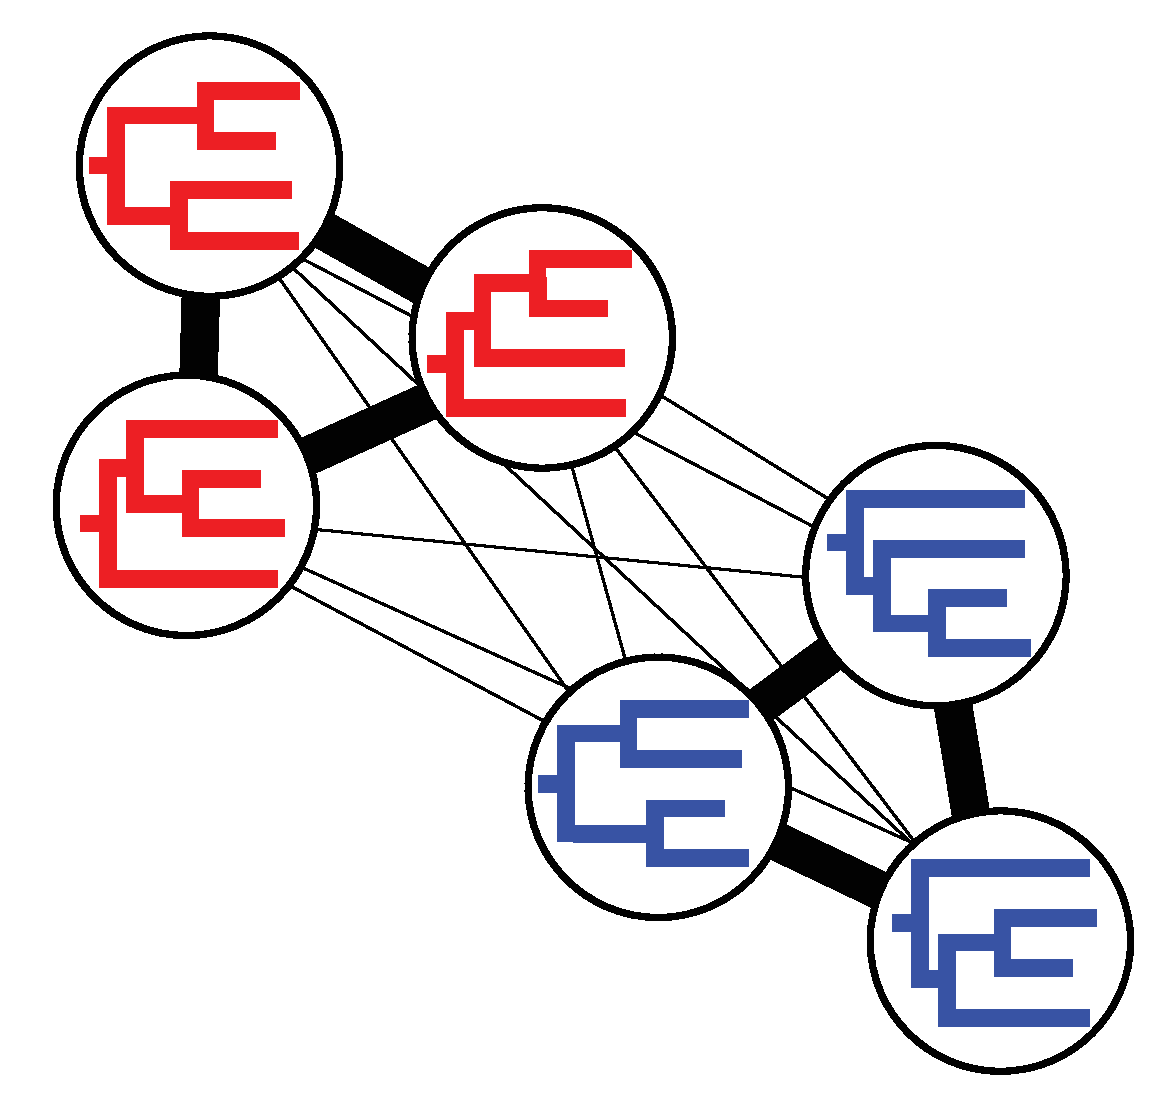
\includegraphics[scale=0.25]{imagesForManual/Figure2.pdf}
\caption{A cartoon topological affinity network. Circles are nodes in the network, each of which corresponds to one tree from a tree set. Edges represent the affinity (or similarity) between the trees, with thicker lines indicating greater affinity. Tree colors correspond to one intuitive definition of communities in this network.}\label{fig2}
\end{figure}


\begin{figure}[thbp!]\centering
\begin{subfigure}{0.4\textwidth}\centering
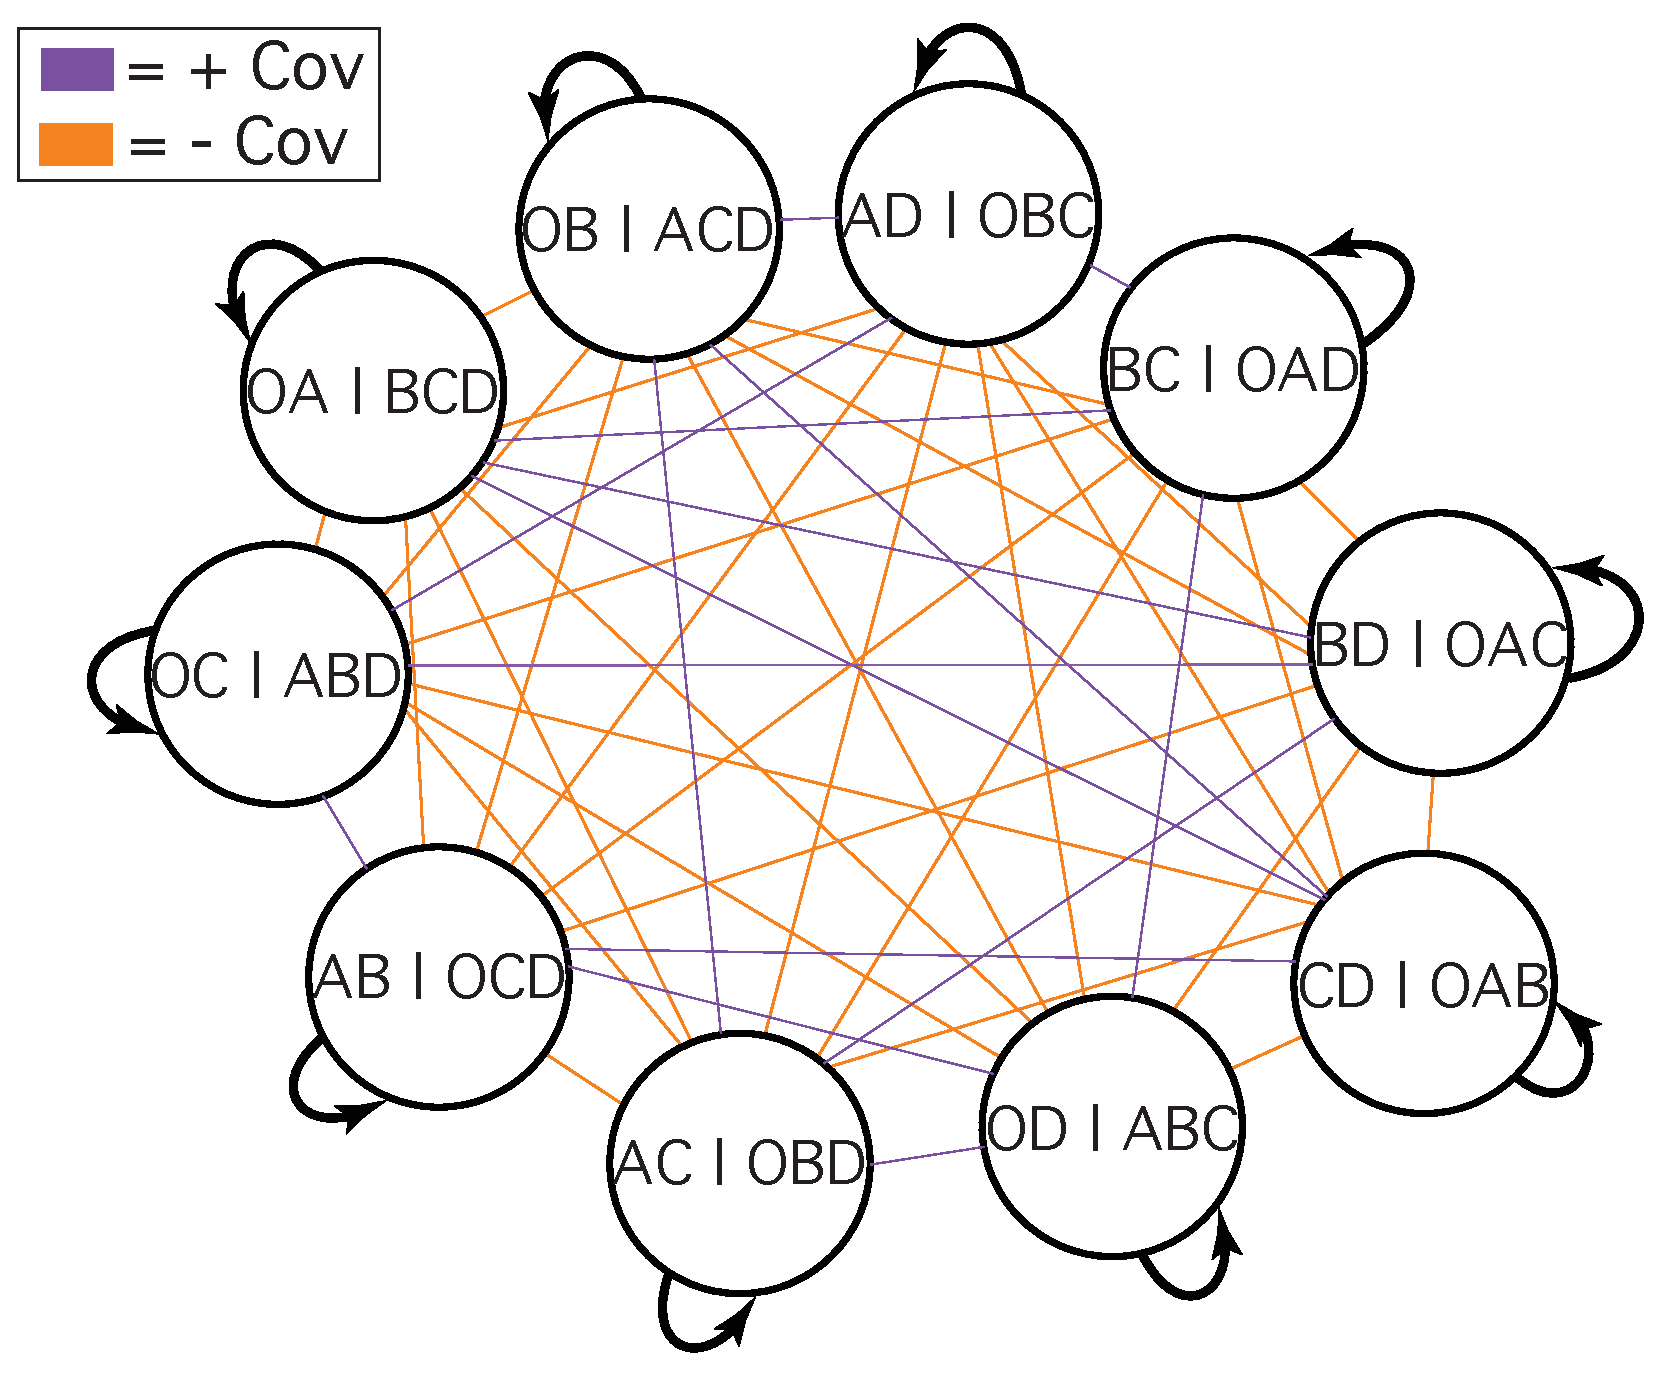
\includegraphics[scale=0.25]{imagesForManual/Figure3a.pdf}
\end{subfigure}
~ % add a little space
\begin{subfigure}{0.4\textwidth}\centering
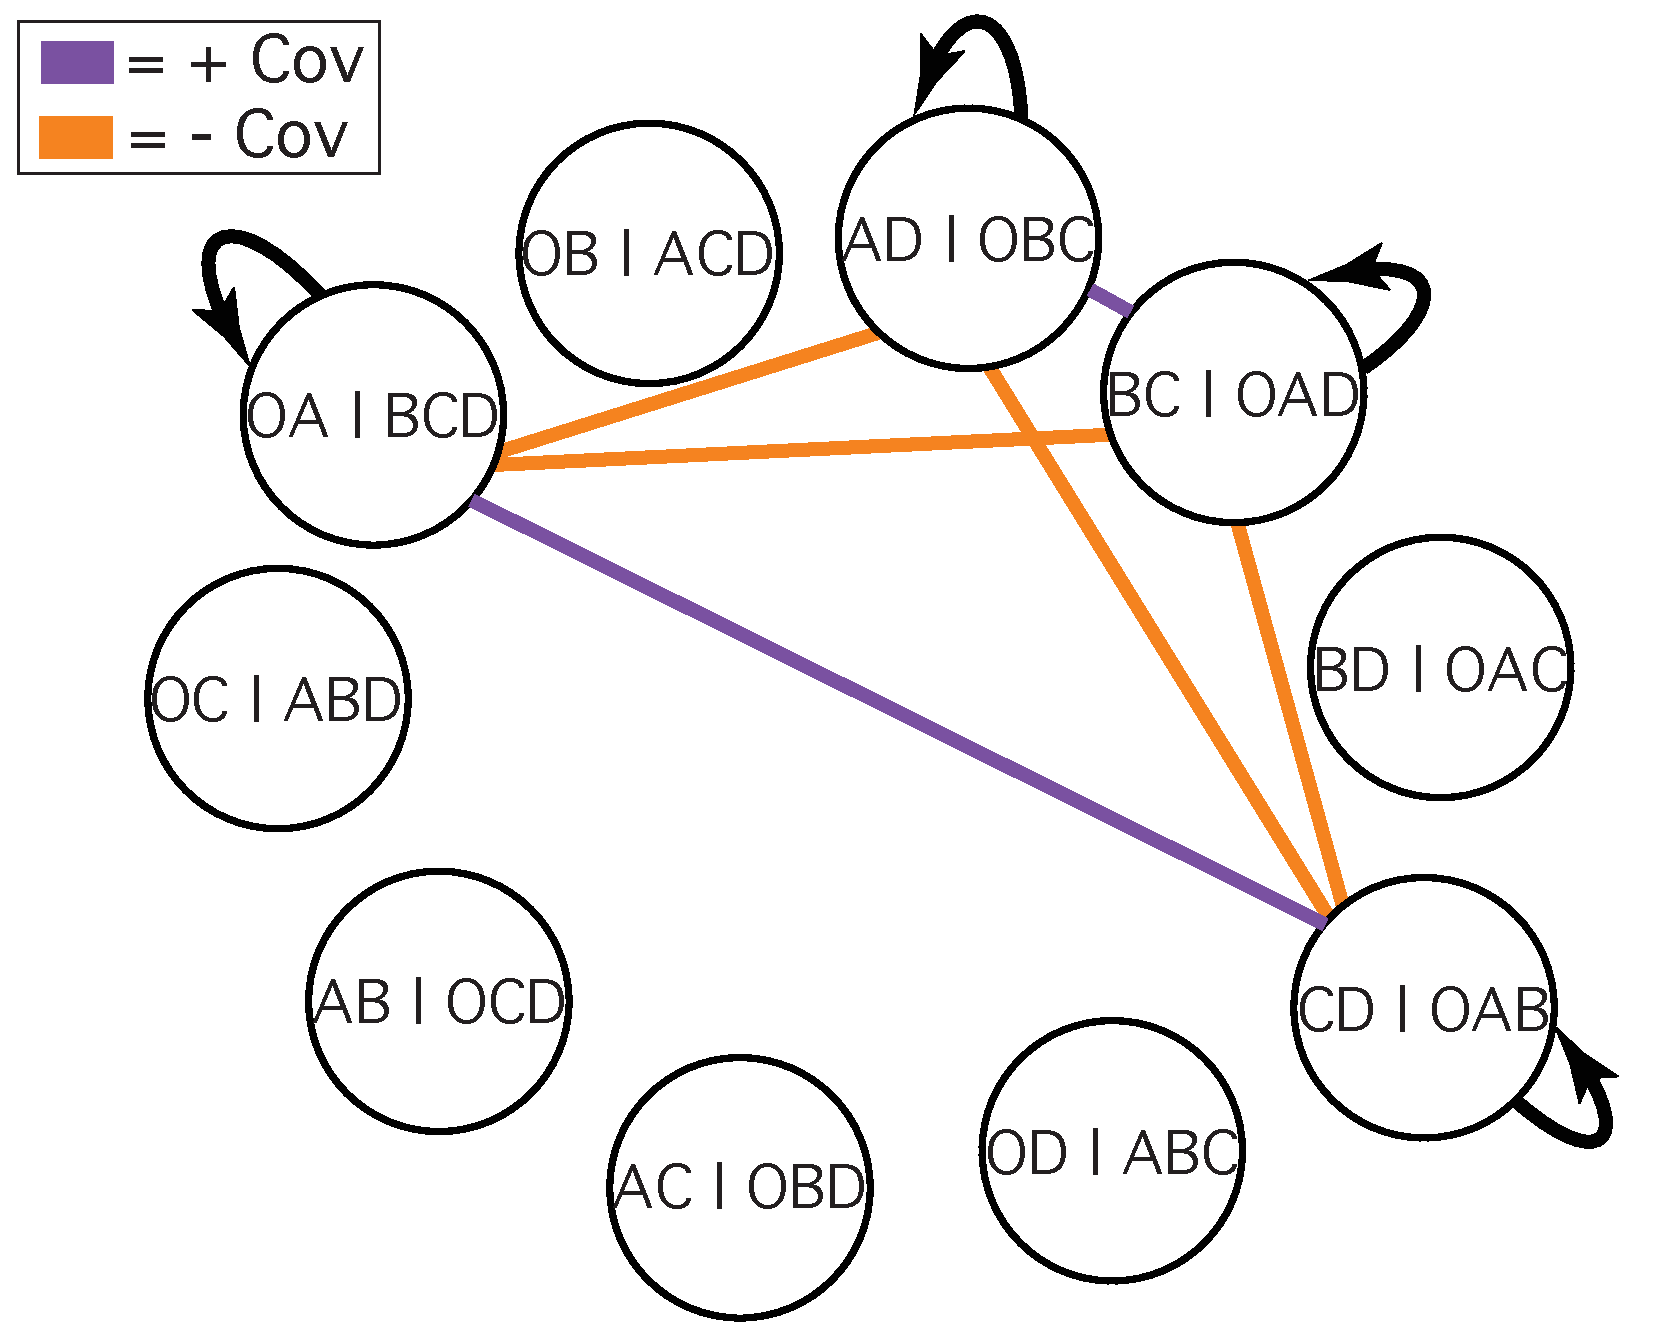
\includegraphics[scale=0.25]{imagesForManual/Figure3b.pdf}
\end{subfigure}

\caption{Two example bipartition covariance networks for sets of unrooted, $5-$taxon trees. The network on the left corresponds to a tree set with a uniform distribution of frequencies across all possible tree topologies. Some weak covariances exist in this network, because some pairs of bipartitions are mutually exclusive and are therefore found together less often than would be expected based on their frequencies alone. The network on the right corresponds to a tree set with only two topologies present at equal frequencies.}\label{fig3}
\end{figure}




%%%%%%%%%%%%%%%%%%%%%%%%%%%%%%%%%%%%%%%%%%%%%%%%%%%
% QUICKSTART TUTORIAL
%%%%%%%%%%%%%%%%%%%%%%%%%%%%%%%%%%%%%%%%%%%%%%%%%%%
\newpage
\section{QUICKSTART TUTORIAL with CLVTreeScaper}\label{sect:QuickstartTutorial}

%%%%%%%%%%%%%%%%%%%%%%%%%%%%%%%%%%%%%%%%%%%%%%%%%%%
% Getting Started
\subsection{Getting Started}\label{subsect:GettingStarted}

%%%%%%%%%%%%%%%%%%%%%%%%%%%%%%%%%%%%%%%%%%%%%%%%%%%
% Installation
\subsubsection{Installation}\label{subsubsect:Installation}

The Quickstart Tutorial uses a command line version(CLV) of TreeScaper with bash interface, which requires users to compile source code for their own machine. There are also pre-compile executable binary for the Mac and Linux abailable from the TreeScaper website at: \\

\noindent{\color{blue}\url{https://github.com/TreeScaper/TreeScaper}} \\

After compiled, put the executable binary {\tt CLVTreeScaper} under the folder with necessary parameter files {\tt nldr\_parameters.csv} and {\tt dimest\_parameters.csv}.\\
%%%%%%%%%%%%%%%%%%%%%%%%%%%%%%%%%%%%%%%%%%%%%%%%%%%
% Example Tree Set
\subsubsection{Example Tree Set}\label{subsubsect:ExampleTreeSet}

The tree set that will be used throughout this tutorial is titled {\tt 1000bp1L.nex}, placed under subfolder {\tt /test/}. The alignment used to generate this set of bootstrap trees was simulated such that half the sites were generated using one topology, while the other half were generated using another. "guide\_tree1.pdf" and "guide\_tree2.pdf" show the two topologies, corresponding to the first and second halves of the alignment, respectively.  Bipartitions that conflict between these topologies are in color.  A bootstrap analysis was then performed in Garli, to produce the $100$ trees in this tree set.  In this tutorial, we will analyze this tree set in TreeScaper to explore the two conflicting signals present in the data. \\



%Basic Computations
\subsection{Basic Computations}\label{subsubsect:BasicComp}

To obtain the bipartitions information of the tree set. Run:\\
{\tt ./CLVTreeScaper -trees -f {test/1000bp1L.nex} -w 0 -r 0}\\
{\tt -o Cova -post test }\\

The output file {\tt Bipartition\_Count\_test.out} is the list of all bipartitions appeared in the tree set with their bitstring representation and appeared times.

The output file {\tt Bipartition\_test.out} is the listed form of the sparse Bipartition matrix.

The output file {\tt Covariance\_test.out} is the covariance matrix of all appeared bipartitions.

To obtain certain kind of tree distance, run:\\
{\tt ./CLVTreeScaper -trees -f {test/1000bp1L.nex} -w 1 -r 0 -dm URF}\\
{\tt -o Dist -post test }\\

The output file {\tt Distance\_test.out} is the unweighted Robinson-Foulds distance matrix of all trees.

To obtain the consensus trees, run:
{\tt ./CLVTreeScaper -trees -f {test/1000bp1L.nex} -w 1 -r 0 }\\
{\tt -o Consensus -post test }\\

The output file {\tt Consensus\_test.out} is the Majority consensus trees in Newick format. 



%%%%%%%%%%%%%%%%%%%%%%%%%%%%%%%%%%%%%%%%%%%%%%%%%%%
% Visualizing Tree Space
\subsection{Visualizing Tree Space}\label{subsect:VisualizeTreeSpace}

In order to visualize the tree set, we perform NLDR to $\mathbb{R}^{n\times 3}$ so that we obtain $n$ points with $3-$tuple of coordinates. Those points generate the Eucldean distance matrix that best approximate the tree distance matrix we obtain from the previous step. To perform the NLDR on tree distance matrix, run
{\tt ./CLVTreeScaper -nldr -f {test/Distance\_test.out} -d 3 -post NLDR\_test}\\

The output file {\tt Coordinates\_NLDR\_test.out} is the coordinates matrix $X\in \mathbb{R}^{n\times 3}$. Each row is a point in $\mathbb{R}^3$ representing one tree. We then may use any convenient plotting software to plot each row of $X$ in $3-$ sapce.

The output file {\tt Distance\_NLDR\_test.out} is the Euclidean distance matrix generated by $X$.


%%%%%%%%%%%%%%%%%%%%%%%%%%%%%%%%%%%%%%%%%%%%%%%%%%%
% Community Detection
% \subsection{Community Detection}\label{subsect:CommunityDetection}


% Before using community detection to identify distinct phylogenetic signals, we need
% to construct networks using our tree set. We will then perform community detection on
% these networks to identify distinct topological signals and the sets of bipartitions that strongly
% conflict between them. As mentioned in the Introduction, TreeScaper uses two types of
% networks: topological affinity and bipartition covariance networks. See above for more detail. \\

% %%%%%%%%%%%%%%%%%%%%%%%%%%%%%%%%%%%%%%%%%%%%%%%%%%%
% % Community Detection on a Topological Network
% \subsubsection{Community Detection on a Topological Network}\label{subsubsect:CommunityDetectionTopologicalNetwork}

% First, we will construct a topological affinity network, where nodes represent
% individual trees in the tree set and edges between these nodes are weighted by the affinity
% between the trees. Since affinities are the converse of distances, we need to convert our
% previously calculated distances to affinities. In the topmost tab menu, go back to the {\it Trees
% and Bipartition Computation} tab. Select \ul{Load/Convert Tree-to-Tree Distances to Affinities}
% from the main dropdown menu in this tab. Select \ul{Unweighted RF-distance} from the {\it Distance
% in Memory} dropdown. Make sure the {\it Affinity Type} is set to \ul{Reciprocal} then click {\bf Affinity}.
% This will calculate the reciprocal of each distance in the distance matrix and use this as a
% measure of affinity, or similarity, between the trees. \\


% Now select the {\it Community Detection} tab at the top and \ul{Community Detection on
% Affinities} from main dropdown menu. \ul{Affinity-URF} should be selected in the "Affinity in
% memory" dropdown. In the "Model Type" dropdown select \ul{Constant Potts Model}, and in
% "Find Plateaus" select "Automatically". Click {\bf Community}. A dialogue box will open that asks you 
% to open a directory. Output files from community detection will be written to this directory. A variety of specific information
% about the community detection analysis is also printed to the log. For now, we will ignore most of
% this information. The basic idea is to vary a tuning parameter (lambda) and see how the
% inferred community structure changes. The preferred community structure is the one that is
% most robust to changes in the tuning parameter. These naturally robust community
% definitions are referred to as plateaus (which will make more sense in a moment). We prefer
% the plateau with the largest "lower bound length" value. This plateau should represent some
% intrinsic community structure of the affinity matrix. \\


% When community detection is finished, click {\bf Plot} to generate a figure showing how
% various summaries of the inferred community structure change with varying values of 
% lambda. For now, we will focus on the "Labels for Communities" line and look for the largest
% flat region (a plateau!) where the community labels remain stable as lambda varies. Note that
% plateaus frequently occur on the left and right ends of these plots, but they represent trivial
% community structures where all nodes are placed in a single community (the left end) or
% every node is assigned to its own unique community (the right end). In this example, the
% plateau of interest occurs when lambda is between $0.6$ and $0.9$. See Section~\ref{subsect:CommunityDetectionMenu} of this manual
% and the Appendix~\ref{appendix:CDModels} for more details on why TreeScaper uses this definition of intrinsic community structure. Pick a $\lambda+$ value in the range of $\lambda+$ values corresponding to the plateau ($0.7$, for example). Returning to the main window, select "Manually" for the "Find Plateaus" option. Set both the "From" and "To" values to the chosen $\lambda+$ value. Click {\bf Community}. The plateau community structure will be printed to the log pane. For now, we are primarily interested in which trees (i.e., nodes in the network) are assigned to each community. \\


% Using the indices of trees assigned to different communities, you can create
% community-specific consensus trees or color points by community assignment in NLDR
% plots. Copy the node indices corresponding to a community (e.g., those numbers that follow
% "Community $1$ includes nodes:" in the log) and create a separate index file for each
% community that has each number on its own line (see the format of "example\_index\_aff1.txt"
% for each affinity community or use the pre-made files, "example\_index\_aff1-3.txt"). Go back
% to \ul{Compute Consensus Tree} under {\it Trees and Bipartition Computation}, select 'index file' in
% "Considered Trees". Then, load an index file for the community of your choice. Click
% {\bf Consensus Tree}, and then {\bf Plot}. The consensus tree for each affinity community should
% provide a sense for its dominant phylogenetic signal. The files,
% "AffinityConsensusCommunity1-3.pdf", show the affinity community consensus trees,
% although the ordering of the three trees is arbitrary. Conflicting bipartitions from the two
% topologies used to simulate the data are in color. \\


% To color points in an NLDR plot by community, create a comma-separated list of the
% indices for that community. Return to the {\it NLDR and Dimension Estimation} tab and click the
% {\bf Plot Parameters} button. Change the number of clusters to $3$. In the box for each cluster
% under {\it Cluster Index} paste the comma-separated list of indices for each community. Press Tab
% after pasting each set of values, then click {\bf Apply} and {\bf Close}. Once back at the NLDR menu,
% click {\bf Plot result}. The new plot should have the same structure as the previous NLDR plot,
% but with points colored as in Fig.~\ref{fig4}. \\

% For extra practice, try redoing community detection with affinities using weighted RF distances. Does the 
% preferred number of communities differ from the analysis using unweighted RF distances? How many large
% plateaus are found? After coloring communities in the NLDR plot also based on weighted RFs, do these results make sense?

% %%%%%%%%%%%%%%%%%%%%%%%%%%%%%%%%%%%%%%%%%%%%%%%%%%%
% % Community Detection on a Bipartition-Covariance Network
% \subsubsection{Community Detection on a Bipartition-Covariance Network}\label{subsubsect:CommunityDetectionBipartCovNetwork}

% Next, we will construct a bipartition covariance network. Go back through the steps
% of Section~\ref{subsubsect:LoadTreesBasicComp} to reload the tree set, with one important difference: {\it do not select the "weighted trees" option}. You should never use weighted trees to compute a covariance matrix, as the computed values will correspond to covariances in branch lengths rather than bipartition presence/absence. When you read the tree set back in without weights, all of the previous
% data structures will automatically be erased. As	before, select \ul{Compute Bipartition Matrix}
% from	the main dropdown menu and	click	{\bf Compute Bipartition-Tree Matrix}. \\


% Now, select \ul{Load/Compute Bipartition Covariances} from the main dropdown, then
% click {\bf Covariance using Bipartition-Tree Matrix}. Alternatively, you have the option to load a
% previously computed covariance matrix at this stage. Once the covariance matrix has been
% created, select the {\it Community Detection} tab at the top and choose \ul{Community Detection on
% Covariances}. The \ul{Covariance Matrix} option should now appear in the "Covariance in
% Memory" dropdown. Set the "High Freq" to $0.95$ and the "Low Freq" to $0.05$. These settings
% will filter out high and low frequency bipartitions, because they are very difficult to assign to
% particular communities. In the "Model Type" dropdown select \ul{Constant Potts Model}, and
% for "Find Plateaus" select "Automatically". Click {\bf Community}. The lambda values used and
% the largest plateaus are output to the log. The largest plateau is the plateau with the largest
% "lower bound length" values. This plateau indicates the intrinsic community structure of the
% covariance matrix. \\


% When community detection is finished, click {\bf Plot} (Fig.~\ref{fig5}). As with community
% detection for affinity networks, this plot will give you an intuitive sense for the most stable
% community structure -- the largest plateau on the "Labels for communities" line. Also as with
% affinity networks, plateaus frequently occur on the left and right ends of these plots, but they
% represent trivial community structures where all nodes are placed in a single community (the
% left end) or every node is assigned to its own unique community (the right end). For this
% example, there is $1$ community in the left trivial plateau and $10$ communities in the right
% trivial plateau.\\ 


% \begin{figure}[thbp!]\centering
% \includegraphics[scale=0.7]{imagesForManual/Figure5.pdf}
% \caption{Example output from automatic community detection on the bipartition
% covariance network discussed in the tutorial. Note the trivial community structures
% represented by the plateaus at $1$ and $10$ communities.}\label{fig5}
% \end{figure}


% Pick a $\lambda+$ value in the range of $\lambda+$ values for the largest non-trivial plateau ($0$, for
% instance). In {\it Find Plateaus} select "Manually". In {\it $\lambda1$ Fixed}, select $\lambda^{-}$ and set the value to $0$. Set both the {\it From} and {\it To} values to be the chosen $\lambda^{+}$ value. Click {\bf Community}. The plateau community structure will be printed to the log. While TreeScaper does not have built-in functionality to visualize bipartition networks and communities, you can examine the bipartition matrix itself to see which bipartitions are assigned to each community. See the
% "Compute Bipartition-Tree Matrix" menu in Section~\ref{subsubsect:CommunityDetectionBipartCovMenu} for an explanation of how to read
% the bipartition matrix output. \\


% The file "1000bp1L\_comKey.out" shows the bipartitions assigned to each community,
% along with their frequencies. Recall that the dataset used to generate this tree set was
% simulated such that half the sites evolved on one topology and the other half evolved along
% another (see "guide\_tree1.pdf" and "guide\_tree2.pdf", respectively, where conflicting
% bipartitions are shown in color). The file "1000bp1LcovarianceNetwork.pdf" contains a
% schematic of the bipartition-covariance network. Node numbers correspond to the numbered
% bipartitions in the guide trees. Blue and green edges indicate positive and negative
% covariances between bipartitions, respectively. Line weights correspond to the magnitude of
% the covariances. Colored circles circumscribe the nodes assigned to each of the detected
% communities. Each community contains the conflicting bipartitions from one of the two
% topologies used in the simulation. Thus, we have identified the conflicting bipartitions that
% define the two distinct topological signals underlying the sites in this alignment. In the
% affinity network, we also identified both of the original tree topologies and a third topology
% that seems to arise when bootstrapped alignments contain balanced mixtures of sites of the
% two types. \\


%%%%%%%%%%%%%%%%%%%%%%%%%%%%%%%%%%%%%%%%%%%%%%%%%%%
% INSTALLATION
%%%%%%%%%%%%%%%%%%%%%%%%%%%%%%%%%%%%%%%%%%%%%%%%%%%
\newpage

\section{INSTALLATION}\label{sect:Installation}

Source code of TreeScaper command-line version for Mac or Linux can be downloaded from \\

\noindent{\color{blue}\url{https://github.com/TreeScaper/TreeScaper}} \\



CLVTreeScaper requires a CLAPACK properly installed and linked on your machine. 
	CLAPACK-3.2.1 has been attached to this repository. You may also download \href{https://www.netlib.org/clapack/}{here}. See detailed instruction on using BLAS library optimized for your machine in 
	CLAPACK/README.install at step (4).
	
	
	
	For a fast default installation, you will need to
	\begin{table}[!h]
		\begin{tabular}{ll}
			- Clone TreeScaper repository from GitHub                   &(see step 1 below)\\
			- Relocate CLAPACK-3.2.1 and modify CLAPACK make.inc file   &(see step 2 below)\\
			- Modify TreeScaper makeCLVTreeScaper.inc file              &(see step 2 below)\\
			- Make CLAPACK library                                      &(see step 3 below)\\
			- Make CLVTreeScaper binary                                 &(see step 3 below)\\
		\end{tabular}
	\end{table}
	
	
	
	\textbf{Procedure for installing CLAPACK.}
	
	
	
	\begin{enumerate}[(1)]
		\item \texttt{git clone https://github.com/TreeScaper/TreeScaper.git} to build 
		the following directory structure:
		
		\begin{table}[!h]
			\begin{tabular}{ll}
				\texttt{TreeScaper/README.install}           &\\

				\texttt{TreeScaper/makeCLVTreeScaper.inc}    &compiler, compile flags and library\\ 
				&definitions for TreeScaper.\\
				\texttt{TreeScaper/CLAPACK-3.2.1/}           &CLAPACK attached in TreeScaper.\\
				\texttt{TreeScaper/CLAPACK-3.2.1/make.inc}   &compiler, compile flags and library\\
				&definitions, for TreeScaper.\\
			\end{tabular}
		\end{table} 
		
		
		\item Move \texttt{/CLAPACK-3.2.1} outside TreeScaper and modify 
		\texttt{/CLAPACK-3.2.1/make.inc}.
		For default installation, you need to only modify the OS postfix name
		\texttt{PLAT} in \texttt{/CLAPACK-3.2.1/make.inc}.
		For advanced installation, please refer to \texttt{/CLAPACK-3.2.1/README.install}
		
		Update the path of CLAPACK:
		\texttt{CLAPPATH} in \texttt{makeCLVTreeScaper.inc}
		and make sure the OS postfix name is consistent with \texttt{CLAPACK} setting,
		i.e. \texttt{PLAT} in \texttt{/CLAPACK-3.2.1/make.inc} and in \texttt{makeCLVTreeScaper.inc}
		must be the same.
		
		==============================================================
		
		(2)' If there is a \texttt{CLAPACK} already built in your machine. Make sure it has
		the following directory structure:
		
		\begin{table}[!h]
			\begin{tabular}{ll}
				\texttt{CLAPACK/BLAS/}       &C source for BLAS\\
				\texttt{CLAPACK/F2CLIBS/}    &f2c I/O functions (libI77) and math functions (libF77)\\
				\texttt{CLAPACK/INSTALL/}    &Testing functions and pre-tested make.inc files\\
				&for various platforms.\\
				\texttt{CLAPACK/INCLUDE/}    &header files - clapack.h is including C prototypes \\
				&of all the CLAPACK routines.\\
				\texttt{CLAPACK/SRC/}        &C source of LAPACK routines\\
			\end{tabular}
		\end{table} 
		
		
		
		
		Update the path of \texttt{CLAPACK}:
		\texttt{CLAPPATH} in \texttt{makeCLVTreeScaper.inc}
		and check the OS postfix name of \texttt{lapack\_XXX.a} and \texttt{blas\_XXX.a} and modify
		\texttt{PLAT} in \texttt{makeCLVTreeScaper.inc}
		
		For example, if the naming is lapack\_MAC.a and lapack\_MAC.a then, modify\\
		\texttt{PLAT = \_LINUX}\\
		in \texttt{makeCLVTreeScaper.inc}. If the naming is \texttt{lapack.a} and \texttt{blas.a}, modify\\
		\texttt{PLAT =}\\
		in \texttt{makeCLVTreeScaper.inc}.
		
		==============================================================
		
		\item Go to TreeScaper directory. To install the CLAPACK,
		run \texttt{make CLAPACK}
		
		To compile the TreeScaper, run \texttt{make} or \texttt{make CLVTreeScaper}.
		
		You may move the binary CLVTreeScaper to other location for your,
		convenience. Make sure you also move the default parameters files 
		nldr\_parameters.csv and dimest\_parameters.csv to maintain the structure:
		
		\begin{table}[!h]
			\begin{tabular}{ll}
				\texttt{/CLVTreeScaper}           &the CLVTreeScaper binary\\
				\texttt{/nldr\_parameters.csv}    &parameters for nldr routines\\
				\texttt{/dimest\_parameters.csv}  &parameters for dimension estimation routines\\
			\end{tabular}
		\end{table} 
		
		
	\end{enumerate}
	
	
	
	

	To obtain the latest stable version of CLVTreeScaper, update the 'master' GitHub branch,
	\begin{enumerate}[1)]
		\item Keep your customized makeCLVTreeScaper.inc file.
		\item  Run \texttt{git pull}
		\item If the makeCLVTreeScaper.inc is overwritten, restore your
		customized version.
		\item If there is no change on CLAPACK side, which is usually the case,
		run \texttt{make} to get the new binary.
	\end{enumerate}
	
	{\bf Note.} There is also a 'test' branch developing new features, working on improvements and fixing certain bugs. The 'test' branch is not guaranteed to be stable. 





%%%%%%%%%%%%%%%%%%%%%%%%%%%%%%%%%%%%%%%%%%%%%%%%%%%
% COMMAND-LINE TREESCAPER
%%%%%%%%%%%%%%%%%%%%%%%%%%%%%%%%%%%%%%%%%%%%%%%%%%%
\newpage


\section{COMMANDS}\label{sect:COMMANDS}

\begin{figure}[thbp!]\centering
\includegraphics[scale=0.4]{imagesForManual/CLVTreeScaper.pdf}
%\caption{}\label{fig17}
\end{figure}

There are three general run modes for the command-line version of TreeScaper
("CLVTreeScaper"). Using one of these five flags as the first command-line argument sets
the mode (e.g., CLVTreeScaper -trees). Note that there are legacy code from previous version that are still functional but no longer suggested to be use any more. Commands and options related to those code are therefore omitted here. For more information on previous version, please refer to \\
{\tt TreeScaperManual\_v2.pdf}.

The current command structure is shown in Fig.\ref{fig:command}, while the previous structure will remain in the TreeScaper binary. 
	

\begin{figure}[thbp!]\centering
	\includegraphics[width=.8\textwidth]{imagesForManual/command.jpg}
	\caption{Command List and routine structure based on file.}
	\label{fig:command}
\end{figure}

New key arguments \texttt{-comm} and \texttt{-aff} are added to TreeScaper. The new structure is centered at files with header information (in order to simplify file names and shorten argument list).
	
\texttt{-aff} and \texttt{-comm} which stand for affinity and community detection are separated from \texttt{-tree}, which now only takes care of computing bipartition matrix, distance matrix and covariance matrix from tree file. Users are now able to perform any modification on output files from \texttt{-tree}, for example, send them to \texttt{-nldr}. Then \texttt{-comm} will take these (modified) files and other necessary information to perform CD methods. The details of these keys are given in below.

\begin{enumerate}[{\bf (1)}]
\item {\tt -trees} 

In this mode, users can compute a majority rule/strict consensus tree, distance matrix,
bipartition matrix, covariance matrix, affinity matrix, or detect communities in an affinity or
covariance network. Relevant arguments include (default option are given in red):
	\begin{description}
	\item[-f:] Provide the name of the file that contains the data

	% \item[-ft:] The file type. Options are:
	% 	\begin{description}
	% 	\item['Trees':] The file contains trees. The tree format can be either Newick or Nexus.
	% 	\item['Dist':] The file contains distance matrix which can be used to compute affinity matrix or communities.
	% 	\item['Cova':] The file contains covariance matrix which can be used to compute communities.
	% 	\end{description}
	
	\item[-w:] Indicate whether trees are weighted. Options are:
		\begin{description}
		\item['1':] weighted
		\item['0':] unweighted
		\end{description}
	
	\item[-r:] Indicate whether trees are rooted. Options are:
		\begin{description}
		\item['1':] rooted
		\item['0':] unrooted
		\end{description}
	
	\item[-o:] This option is used to indicate what output the user is interested in. Options are:
		\begin{description}
			% \item['BipartMatrix']
			\item['Consensus']
			\item['Dist']
			% \item['Affinity']
			\item['Cova']
			% \item['Community']
		\end{description}

	\item[-post:] Suffix name of file. Options are:
		\begin{description}
			\item['none'] 
			\item['time']
			\item['AnyOtherString':] filename will be attached with {\tt \_AnyOtherString}  
		\end{description}
	\end{description}

\vspace{0.5cm}

When outputting a bipartition matrix (-o BipartMatrix):
	\begin{description}
	\item[-bfm:] Bipartition matrix output type. Options are: 
		\begin{description}
		\item['list':] Output sparse matrix in the form (row, column, value)
		\item['matrix':] Output as if it is a full matrix
		\end{description}
	\end{description}
	
\vspace{0.5cm}
		
When computing a majority-rule or strict consensus tree (-o Consensus), use the -if, -ct,
and/or -cfm flags:
	\begin{description}
	\item[-if:] The name of a list file. Consensus tree computations will only consider the trees indicated in the file.
	
	\item[-ct:] The type of consensus tree to be computed. Options are:
		\begin{description}
		\item['Majority':] Majority consensus tree
		\item['Strict':] Strict consensus tree
		\end{description}
	
	\item[-cfm:] Format of the consensus tree file. Options are:
		\begin{description}
		\item['Newick']
		\item['Nexus']
		\end{description}
	\end{description}

\vspace{0.5cm}
	
When computing a distance matrix (-o Dist):
	\begin{description}
	\item[-dm:] Indicates the distance metric. Options are:
		\begin{description}
		\item['URF':] Unweighted Robinson-Foulds distance
		\item['RF':] Weighted Robinson-Foulds distance
		\item['Mat':] Matching distance
		\item['SPR':] Subtree-Prune-Regraft
		\end{description}
	\end{description} 

\vspace{0.5cm}




\ul{\bf Examples of command-line runs}
{\it Options specified by the are given inside braces. When specific alternatives are available, they
are separated by commas (e.g., \{option1,option2\}). When numbers can be specified anywhere in
a continuous range, the bounds of the range are separated by a dash (e.g., \{0-1\}).} \\


% {\it Compute a Bipartition Matrix:} \\
% ./CLVTreeScaper -trees -f {trees.txt} -ft Trees -w {1,0} -r {1,0} -o BipartMatrix -bfm
% \{list,matrix\} \\


{\it Compute a Consensus Tree:} \\
{\tt ./CLVTreeScaper -trees -f \{trees.txt\} -w \{1,0\} -r \{1,0\}}\\
{\tt  -o Consensus -if IndicesFileName -ct \{Majority,Strict\} }\\
{\tt -cfm \{Newick,Nexus\} -post \{none, time, AnyString\}} \\


{\it Compute Distance Matrix:} \\
{\tt ./CLVTreeScaper -trees -f \{trees.txt\} -w \{1,0\} -r \{1,0\}}\\
{\tt  -o Dist -dm \{URF,RF,Mat,SPR\} -post \{none, time, AnyString\}} \\


% {\it Compute Affinity Matrix:} \\
% ./CLVTreeScaper -trees -f \{trees.txt\} -ft Trees -w \{1,0\} -r \{1,0\} -o Affinity -dm \\
% \{URF,RF,Mat,SPR\} -am \{Exp,Rec\} \\


{\it Compute Covariance Matrix:} \\
{\tt ./CLVTreeScaper -trees -f \{trees.txt\} -w \{1,0\} -r \{1,0\} }\\
{\tt  -o Cova -post \{none, time, AnyString\}} \\


\item {\tt -nldr}

In this mode, users can project distance matrix into lower dimensional space using non-linear
dimensionality reduction (NLDR). Relevant arguments include (default option are given in red):
	\begin{description}
	\item[-f:] Name of the file containing distance data.
	
	\item[-t:] The type of distances contained in the file. Options are:
		\begin{description}
		\item['DIS':] A lower triangle matrix of original distances
		\item['COR':] Low-dimensional Euclidean coordinates (if already computed).
		\end{description}
	
	\item[-d:] The desired dimension of the Euclidean representation (usually 1, 2, or 3).
	
	\item[-c:] The chosen cost function. Options are:
		\begin{description}
		\item['CLASSIC\_MDS']
		\item['KRUSKAL1']
		\item['NORMALIZED']
		\item['SAMMON']
		\item['CCA']
		\end{description}
		
	\item[-a:] The chosen NLDR algorithm. Options are:
		\begin{description}
		\item['LINEAR\_ITERATION']
		\item['MAJORIZATION']
		\item['GAUSS\_SEIDEL']
		\item['STOCHASTIC']
		\end{description}
		
	\item[-i:] The method for generating initial Euclidean coordinates. Options are:
		\begin{description}
		\item['RAND':] Randomly choose coordinates for each point.
		\item['CLASSIC\_MDS':] Generate initial coordinates using classic multi-dimensional scaling (MDS).
		\end{description}
	
	
	\item[-s:] A random seed, if initial coordinates are generated randomly.
	
	\item[-post:] Suffix name of file. Options are:
		\begin{description}
			\item['none'] 
			\item['time']
			\item['AnyOtherString':] filename will be attached with {\tt \_AnyOtherString}  
		\end{description}

	\end{description}

\vspace{0.5 cm}	
	
\ul{\bf Example command:}\\
{\tt ./CLVTreeScaper -nldr -f \{test.out\} -t \{DIS,COR\} -d \{AnyPositiveInteger\} }\\
{\tt -c \{CLASSIC\_MDS,KRUSKAL1,NORMALIZED,SAMMON,CCA\} }\\
{\tt -a \{LINEAR\_ITERATION,MAJORIZATION,GAUSS\_SEIDEL,STOCHASTIC\} }\\
{\tt -i \{RAND,CLASSIC\_MDS\} -s 1 -post \{none, time, AnyString\}}\\

\item {\tt -aff}

In this mode, users can process (pre-)adjacency matrix. Relevant arguments include (default option is colored in red):
\begin{description}
	\item[-f:] Provide the name of the file that contains the data

% \item[-ft:] The file type. Options are:
% 	\begin{description}
% 	\item['Trees':] The file contains trees. The tree format can be either Newick or Nexus.
% 	\item['Dist':] The file contains distance matrix which can be used to compute affinity matrix or communities.
% 	\item['Cova':] The file contains covariance matrix which can be used to compute communities.
% 	\end{description}
	\item[-am:] Indicates the distance to affinity transformation. Options are:
	\begin{description}
		\item['Rec':] Reciprocal
		\item['Exp':] Exponential
	\end{description}

	\vspace{0.5cm}

	\item[-post:] Suffix name of file. Options are:
		\begin{description}
			\item['none'] 
			\item['time']
			\item['AnyOtherString':] filename will be attached with {\tt \_AnyOtherString}  
		\end{description}
\end{description}
\vspace{0.5cm}

\item {\tt -comm} 

In this mode, user can preform community detection method on adjacency matrix. Relevant arguments include (default option is given in red):
	\begin{description}
	
		\item[-cm:] Model used to compute communities. Options are:
			\begin{description}
				\item['CNM':] Configuration Null Model
				\item['CPM':] Constant Potts Model
				\item['ERNM':] Erdos-Renyi Null Model
				\item['NNM':] No Null Model
			\end{description}
	
		\item[-lm:] Method of plateau detection. Options are:
			\begin{description}
				\item['auto':] automatically choose lambdas and find plateaus
				\item['manu':] specify intervals by users to find plateaus
			\end{description}

		\item[-post:] Suffix name of file. Options are:
			\begin{description}
				\item['none'] 
				\item['time']
				\item['AnyOtherString':] filename will be attached with {\tt \_AnyOtherString}  
			\end{description}

	\vspace{0.5cm}

\vspace{0.5cm}
	\end{description}

	The following flags are used to specify values of lambda for manual searches:
	\begin{description}
	\item[-lp:] Specify a fixed value of $\lambda^{+}$. Must be between 0 and 1. Used when -lpiv is zero (see below).
	
	\item[-lps, -lpe, -lpiv:] Starting, ending, and sampling intervals for $\lambda^{+}$. Used to explore a range of possible values for $\lambda^{+}$.
	
	\item[-ln:] Specify a fixed value of $\lambda^{-}$. Must be between $0$ and $1$. Used when -lniv is zero (see below).
	
	\item[-lns, -lne, -lniv:] Starting, ending, and sampling intervals for $\lambda^{-}$. Used to explore a range of possible values for $\lambda^{-}$. \\

{\it Note: Either $\lambda^{+}$ or $\lambda^{-}$ must be fixed, because plateau detection is undefined when both vary.} \\

	\item[-hf:] Frequency upper bound. A number between $0$ and $1$. Nodes with frequencies
above this value are ignored.

	\item[-lf:] Frequency lower bound. A number between $0$ and $1$. Nodes with frequencies
below this value are ignored.
	\end{description}

\vspace{0.5cm}

\ul{\bf Examples of command-line runs}
{\it Options specified by the are given inside braces. When specific alternatives are available, they
are separated by commas (e.g., \{option1,option2\}). When numbers can be specified anywhere in
a continuous range, the bounds of the range are separated by a dash (e.g., \{0-1\}).} \\

{\it Compute Communities with $\lambda^{+}$ Fixed:} \\
{\tt ./CLVTreeScaper -comm -f \{Adjacency.out\} -cm \{CNM,CPM,ERNM,NNM\}} \\
{\tt -lm manu -lp \{AnyNumber\} -lns \{AnyNumber\} -lne \{AnyNumber\}} \\
{\tt -lniv \{AnyNumber\} -hf \{0-1\} -lf \{0-1\} -post \{none, time, AnyString\}}\\

{\it Compute Communities with $\lambda^{-}$ Fixed:} \\
{\tt ./CLVTreeScaper -comm -f \{Adjacency.out\} -cm \{CNM,CPM,ERNM,NNM\}}\\
{\tt -lm manu -ln \{AnyNumber\} -lps \{AnyNumber\} -lpe \{AnyNumber\}}\\
{\tt -lpiv \{AnyNumber\} -hf \{0-1\} -lf \{0-1\} -post \{none, time, AnyString\}}\\


{\it Compute Communities with Automatically Chosen Lambdas:} \\
{\tt ./CLVTreeScaper -comm -f \{Adjacency.out\} -cm \{CNM/CPM/ERNM/NNM\} }\\
{\tt -lm auto -hf \{0-1\} -lf \{0-1\} -post \{none, time, AnyString\}} \\


\item {\tt -dimest}

In this mode, users can estimate the intrinsic dimensionality of their data. This estimate can
help in deciding on an appropriate number of dimensions to use when performing NLDR
projections.
	\begin{description}
	\item[-f:] Name of the file containing distance data.
	
	\item[-i:] The type of distances contained in the file. Options are:
		\begin{description}
		\item['DIS':] A lower triangle matrix of original distances
		\item['COR':] Low-dimensional Euclidean coordinates (if already computed).
		\end{description}
	
	\item[-e:] The chosen estimator. Options are:
		\begin{description}
		\item['CORR\_DIM':] Correlation dimension estimator
		\item['NN\_DIM':] Nearest neighbor estimator
		\item['MLE\_DIM':] Maximum likelihood estimator
		\end{description}
	\end{description}

\ul{\bf Example command:}\\
{\tt ./CLVTreeScaper -dimest -f \{test.out\} -i \{DIS,COR\}}\\
{\tt  -e \{CORR\_DIM,NN\_DIM,MLE\_DIM\}} \\
\end{enumerate}

%%%%%%%%%%%%%%%%%%%%%%%%%%%%%%%%%%%%%%%%%%%%%%%%%%%
% APPENDIX (COMMUNITY DETECTION MODELS)
%%%%%%%%%%%%%%%%%%%%%%%%%%%%%%%%%%%%%%%%%%%%%%%%%%%
\newpage
\appendix
\section{UTILITY DETAILS}\label{appendix:UTILITYDETAILS}

The command-line version of TreeScaper (CLVTreeScaper) has three independent major routines implemented, computing tree-related objects, computing NLDR and performing community detection. A comprehensive task, e.g. visualizing trees grouped by their distance, will need a sequence calls to CLVTreeScaper for activating different routines. These routines communicate with each other and carry out essential information through the output-input files.

\noindent \ul{\bf Input-Output files:}
\begin{table}[thbp!]\centering
	\begin{tabular}{|c|l|l|}
		\hline
		Command key & Input& Output \\
		\hline
		{\tt -trees} & Nexus formatted trees & Bipartition list\\
		& Newick formatted trees & Bipartition covariance $K$\\
		& & Distance matrix of trees $D\in \mathbb{R}^{n\times n}$\\
		& & Consensus trees\\
		\hline
		{\tt -nldr} & Distance matrix $D\in \mathbb{R}^{n\times n}$ & Distance matrix $\bar{D}$ from Euclidean $\mathbb{R}^k$\\
		& Coordinates matrix $X\in \mathbb{R}^{n\times m}$ from $\mathbb{R}^m$& Coordinates matrix $\bar{X}\in \mathbb{R}^{n\times k}$ from $\mathbb{R}^k$\\
		&&Information of NLDR quality\\
		\hline
		{\tt -aff}\footnote{This command now only takes in distance matrix and convert it to an affinity matrix. In the furture it will get expanded as command with different ways of preprocessing general adjacency matrix} & (pre)-Adjacency matrix $\text{Adj}\in \mathbb{R}^{n\times n}$ & Adjacency matrix $\widetilde{\text{Adj}}\in \mathbb{R}^{n\times n}$\\
		\hline
		{\tt -comm} & Adjacency matrix $\text{Adj}\in \mathbb{R}^{n\times n}$ & Modularity and grouped nodes' ID\\
		\hline
	\end{tabular}
\end{table}

Particular information can be carried out through different calls of CLVTreeScaper by the header information included in files. Note that {\tt -trees} command does not yet support header information in tree file due to some comflict of formatting.

An header information is a collection of messages surrounded by angle bracket {\tt < >}. Each line inside the bracket separated by {\tt :} is a message in forms of {\tt item:content}. Some message, abou labeling created time or output format, will be updated and the rest will be carried out in the output file generated by CLVTreeScaper.



Bipartitions and related objects are the basis objects for computing further objects. Given a set of trees with exactly $n$ leaves, CLVTreeScaper generates an unique ID for each possible bipartition as $n$ bitstring. See \cite{sul2011big} about details of the translation.

\subsection{Computing bipartitions and their distribution}

When CLVTreeScaper {\tt -trees} is called, it will read trees from file and store all of them in memory.\footnote{In the future, we can develop functionality that allow to store limited trees in case the tree set is to big to store.} 

Then it scan through the tree set and record every bipartition presented in the tree set. For this tasks, CLVTreeScaper first assigns hash values to each leaf and then performs the following subroutine so that 

\begin{algorithm}[H]
    \DontPrintSemicolon
    \KwIn{Tree with leaves $\{l_i\}, i =1,\cdots,n$}
    \KwOut{Critial point $p_*$ of $f$}
    \KwData{Hash values of each leaf $\{h_i^1\},\{h_i^2\},i =1,\cdots,n$}
    $i=0$ \;
    \While{Scanning with in-order travelsal}    
    { 
		\If{The current node is $l_i$}
		{
			Assign hash value $h_i^1,h_i^2$ to the node\;
			Generate bitstring "$\delta_{1i}\cdots\delta_{ni}$" and assigned to the node\;
		}
		\Else{
			Assign the sum of hash values accordingly of its children to the node\;
			Generate bitstring by bit-wise OR operation to its children's bitstring and assigned to the node\;
		}
	}
	Label the bitstring of the root by its two hash values and stored it in hash table\;
    \caption{Compute hash value of bipartition}
    \label{alg:computehash}
\end{algorithm}

After performing Alg. \ref{alg:computehash}, the root has hash value that label the corresponding to the bitstring for its bipartition structure.

Once every tree has been processed, CLVTreeScaper will scan through tree set again but only access every trees root's hash value. By storing and sorting hash values of the root, CLVTreeScaper is then able to count how many times bipartitiond are appeared in this tree set (via looking through hash table). 

{\bf Complexity concern:} sorting is not necessary especially when number of bipartition is far smaller than the number of trees.

{\bf Data storage concern:} The structure of hash table is poorly managed. It is a $3-$ dimensional array by construction, i.e., uses $3$ labels, yet only two indices are labeled on the data, bipartitions labeled by bitstring and trees labeled by their ID. It costs unnessary and complicated code as well as inconsistent coding when the extra label is flatten for the computation of weighted RF-distance.



\subsection{Computing tree distances}

CLVTreeScaper supports computation of 3 kinds of tree distance: Robinson Foulds distance\footnote{\href{https://en.wikipedia.org/wiki/Robinson-Foulds_metric}{wiki page of Robinson Foulds distance}}, (URF) for unweighted tree and (RF) for weighted tree, Matching distance (Mat) and subtree-Prube-and-Regraft (SPR) distance. CLVTreeScaper implements RF-distance and Matching distance with its original code and use the SPR-tree library developed by for the computation of SPR-distance.

\subsubsection{Robinson Foulds distance} 

For unweighted trees $t_i$ and $t_j$, let $A_i$, and $A_j$, be the number of all bipartitions that the structure of $t_i$, and $t_j$ accordingly, can obtain. Let $B_{ij}$ be the number of bipartition appeared in both $t_i$ and $t_j$. Then the RF-distance is given by
\begin{equation}\label{eq:URF-distance}
	d^{\text{URF}}(t_i,t_j) = \frac{A_i+A_j- 2B_{ij}}{2}.
\end{equation}
For weighted trees $t_i$ and $t_j$, let $\{b_k\}$ be all bipartitions appeared in at least one of them. Let $w_{i}(b_k)$ and $w_{j}(b_k)$ be the weight of root which correspond to an instance of bipartition $b_k$ in tree $t_i$ and $t_j$. (If there is no instance of $b_k$, then it is zero.) Then the RF distance is given by
\begin{equation}\label{eq:RF-distance}
	d^{\text{RF}}(t_i,t_j) =\frac{\sum_{b_k}|w_i(b_k)-w_j(b_k)| + |w_j(b_k)-w_i(b_k)|}{4}
\end{equation}
{\bf Algorithmic concern:} why not compute the equivalent $\sum_{b_k}|w_i(b_k)-w_j(b_k)|/2$ instead?

The computation is done on single precision floating point system.

\subsubsection{Matching distance} 

In order to compute matching distance, an combinatorial optimization problem will be formed for each pair of trees $(t_i, t_j)$ first, then Hungarian algorithm\footnote{\href{https://en.wikipedia.org/wiki/Hungarian_algorithm}{wiki of Hungarian algorithm}} implemented in \cite{stachniss2004c} is called. The matching distance is the solution to the optimization problem.

The cost matrix $C$ is describing the bitwise distance between bipartition $b_k$ and $b_l$ that appeared in at least one of the two trees. Let $\Delta_{kl}$ be the number of different bits in bitstring of $b_k$ and bitstring of $b_l$ (for bipartition never appear in a tree, make the bitstring all {\tt 1}). $C_{kl}$ is given by
\begin{equation}\label{eq:Mar-distance-cost}
	C_{kl} = \min(\Delta_{kl}, N_{\text{taxa}} - \Delta_{kl})
\end{equation}
where $ N_{\text{taxa}}$ is the number of taxa. 
Then distance is given as
\begin{equation}\label{eq:Mar-distance}
	d_{ij}^{\text{Mat}} = \min_{P \text{ is Permutation}} \text{Tr}(PCP^T).
\end{equation}
Note that the problem scale $M$ is the number of all possible bipartitions and complexity of Hungarian algorithm is at $O(M^3)$. There are $n(n-1)/2$ distance needed to be computed, leading to overall complexity $O(n^2M^3)$

{\bf Algorithmic Error:} In handling the case where $b_k$ is not in tree $t_i$ or $b_l$ is not in tree $t_j$, the code calling  {\tt onebitstrXOR} is not comparing to {\tt 1} bitstring.

\subsubsection{subtree-Prube-and-Regraft distance} 

TreeScaper implements routine to translate the tree structure it created to SPR tree structure implemented in Chris Whidden's library\footnote{The library can be found in his \href{https://web.cs.dal.ca/~whidden/}{homepage}}. In addition, CLVTreeScaper calls the routines built-in that library for computing SPR distance. Details of the algorithm implemented in Whidden's library can be found in \cite{whidden2018calculating}.

{\bf Algorithmic concern:} TreeScaper may implement SPD distance computation itself in the future.

\subsection{Computing NLDR of distance matrix}

For the task of NLDR, there are 5 iterative methods implemented for nontrivial stress function and 1 deterministic method implemented for MDS cost fucntion. 

{\bf Data storage concern:} All symmetric matrix are stored in dense form.

{\bf Complexity concern:} The update is on the coordinate matrix $X\in \mathbb{R}^{n\times k}$ at the scale of $O(nk)$ but the stress function evaluated at $D\in \mathbb{R}^{n\times n}$ at the scale of $O(n^2)$, which implies forming $D_i$ with complexity $O(nk^2)$ and evaluating stress function $O(n^3)$ is necessary at each step. Is there a way to work directly on $X$, which get rid of $O(nk^2)$ of forming $D$ and get less computation $O(nk^2)$ for evaluating cost function.

\subsubsection{Classic multidimensional scaling(MDS)} 

This method, also known as standard scaling method\footnote{\href{https://en.wikipedia.org/wiki/Multidimensional_scaling}{wiki of multidimensional scaling.}}, only applies to Euclidean distance matrix. However, this method also used as a lousy solution for initial guess of other problem.

For given distance matrix $D\in \mathbb{R}^{n\times n}$ or coordinates matrix $C\in \mathbb{R}^{n\times m}$ from $\mathbb{R^{k}}$, compute the squared proximity matrix $D^{(2)} = \begin{bmatrix}
	d^2_{ij}
\end{bmatrix}$ and CLVTreeScaper performs the following algorithm.
\begin{algorithm}[H]
    \DontPrintSemicolon
    \KwIn{Squared proximity matrix $D^{(2)}$, targeted dimension $k$}
    \KwOut{Coordinate matrix $X\in \mathbb{R}^{n\times k}$}
    Perform singular value decomposition of $D^{(2)}=U\Sigma V^T$\;
	Selete $k$-th positive largest eigenvalue $\lambda_i$ and their eigenvectors $U_i$\;
	Form coordinate matrix by lining up scaled eigenvectors $\begin{bmatrix}
		\lambda_1^{1/2}U_1&\cdots& \lambda_k^{1/2}U_k
	\end{bmatrix}$
    \caption{Multidimensional Scaling}
    \label{alg:MDS}
\end{algorithm}

Note that negative eigenvalue only appear when distance matrix is not Eculidean.



{\bf Algorithmic concern:} It perform SVD on dense symmetric matrix, instead of eigenvalue decomposition.

\subsubsection{Linear iteration} 

Linear iteration method is straight-forward. For different cost functions, there are subroutines built in CLVTreeScaper to obtain a descent direction (usually the negative gradient) and then CLVTreeScaper performs the following algorithm

\begin{algorithm}[H]
    \DontPrintSemicolon
    \KwIn{Initial guess $X_0\in \mathbb{R}^{n\times k}$}
	\KwOut{Coordinate matrix $X\in \mathbb{R}^{n\times k}$}
	\KwData{Subroutine $f$ for computing descent direction, step size $\lambda$}
	$i\gets 0$\;
    \While{not converged}{
		$V_i\gets f(X_i)$\;
		$X_{i+1}\gets X_i + \lambda V_i$\;
		$i\gets i+1$\; 
	}
    \caption{Linear Iteration}
    \label{alg:LinearIteration}
\end{algorithm}

{\bf Algorithmic concern:} Linear iteration uses fixed stepsize. There are better stepsizes, e.g., Armijo stepsize.


\subsubsection{Gauss-Seidel} 

Gauss-Seidel methods is similar to linear iteartion, except that it perform changes on entry-wise basis of the coordinate matrix $X_i$.

\begin{algorithm}[H]
    \DontPrintSemicolon
    \KwIn{Initial guess $X_0\in \mathbb{R}^{n\times k}$}
	\KwOut{Coordinate matrix $X_*\in \mathbb{R}^{n\times k}$}
	\KwData{Subroutine $f$ for computing descent direction, step size $\lambda$}
	$l\gets 0$\;
    \While{not converged}{
		$X_{l+1}\gets X_l$ (No computation exists in here)\;
		$i\gets 1$\;
		$j\gets 1$\;
		\For{$i\leq n$}
		{
			\For{$j\leq k$}
			{
				Compute descent direction $V_{l,ij}$ along $X_{l,ij}$\;
				Find Armijo stepsize $\lambda_{l,ij}$\;
				$X_{l+1,ij}\gets X_{l+1,ij} + \lambda_{l,ij}V_{l,ij}$\;
				$j\gets j+1$\;
			}
			$i\gets i+1$\;
		}
		$l\gets l+1$\;
	}
    \caption{Gauss-Seidel}
    \label{alg:GaussSeidel}
\end{algorithm}


\subsubsection{Stochastic} 

Stochastic methods refers to the stochastic descent method\footnote{\href{https://en.wikipedia.org/wiki/Stochastic_gradient_descent}{wiki of stochastic descent method}}, which selects random set of coordinates $X_{i_{l}j_{l}}$ and compute descent direction along them. The ratio between number of selected indices and number of all indices is control by parameter {\tt epochs}. The stepsize is control by parameter {\tt STO\_alphan}.


\begin{algorithm}[H]
    \DontPrintSemicolon
    \KwIn{Initial guess $X_0\in \mathbb{R}^{n\times k}$}
	\KwOut{Coordinate matrix $X_*\in \mathbb{R}^{n\times k}$}
	\KwData{Subroutine $f$ for computing descent direction, stepsize $\{\lambda_m\}_{m=1}^{M}$}
	$l\gets 0$\;
    \While{not converged}{
		$X_{l+1}\gets X_l$ (No computation exists in here)\;
		Sample $\{i_m,j_m\}_{m=1}^{M}$\;
		$m\gets 0$\;
		\For{$m\leq M$}{
			Compute descent direction $V_{l,m}$ along selected indices $\{i_m,j_m\}$ \;
			$X_{l+1}\gets X_{l+1} + \lambda_{m}V_{l,m}$\;
			$l\gets l+1$\;
			$m\gets m+1$\;
		}
	}
    \caption{Stochastic}
    \label{alg:Stochastic}
\end{algorithm}

{\bf Algorithmic concern:} fixed stepsize is used.

\subsubsection{Metropolis} 

This algorithm refers to Metropolis-Hastings algorithm\footnote{\href{https://en.wikipedia.org/wiki/Metropolis-Hastings_algorithm}{wiki of Metropolis-Hastings algorithm}}, which samples descent vector $V$ around the gradient descent direction, accepts/rejects it by the decrease in $f$ obtained along $V$.

\begin{algorithm}[H]
    \DontPrintSemicolon
    \KwIn{Initial guess $X_0\in \mathbb{R}^{n\times k}$}
	\KwOut{Coordinate matrix $X_*\in \mathbb{R}^{n\times k}$}
	\KwData{Subroutine $f$ for computing gradient descent direction}
	$i\gets 0$\;
	$j\gets 0$\;
	\While{$X_j$ not converged}{
		Compute $\nabla_j = -\text{grad} f(X_j)$\;
		Compute stepsize $\lambda_j = 1/\|\nabla_j\|_F^2$\;
		\While{Not enough decrease in $f$ at $X_{j,i}$ and $i<2000$}{
			Sample $V_i$ around $\nabla_j$\;
			$X_{j,i}\gets \lambda_jV_i$\;
			$i\gets i+1$\;
		}
		$X_{j+1}\gets X_{j,i}$\;
		$j\gets j+1$
	}
    \caption{Metropolis}
    \label{alg:Metropolis}
\end{algorithm}

\subsubsection{Majorization} This algorithm refers to Majorize-Minimization algorithm\footnote{\href{https://en.wikipedia.org/wiki/MM_algorithm}{wiki of MM algorithm.}}, which construct a surrogate funtion represented by $B_i\in \mathbb{R}^{n\times n}$ from $D_i=\text{Dist}(X_i)$ the distance matrix of coordinates $X_i$. The optimal solution for $B_i$ is known and given by $f$. 

\begin{algorithm}[H]
    \DontPrintSemicolon
    \KwIn{Initial guess $X_0\in \mathbb{R}^{n\times k}$}
	\KwOut{Coordinate matrix $X_*\in \mathbb{R}^{n\times k}$}
	\KwData{Subroutine $f$ for formming related problem $B_i$, $g$ for solving of related problem}
	$i\gets 0$\;
    \While{not converged}{
		Compute $B_i = f(D_i)$\;
		Compute $V_i = g(B_i)$\;
		Update $X_{i+1} \gets X_i + V_i$\;
		Update $D_{i+1}$\;
		$i\gets i+1$\;
	}
    \caption{Majorization}
    \label{alg:Majorization}
\end{algorithm}

{\bf Algorithmic concern:} $D_{i}$ is never updated for NORMALIZED cost function. It seems never converge.

\subsubsection{Stress functions} 

TreeScaper implement 4 kinds of stress functions evaluated at distance matrix $D$. NLDR is done by applying specific algorithms above to minimize these cost functions. Under the sense of thses stress functions, the resulted coordiantes $X_*\in \mathbb{R}^{n\times k}$ is said to be the best approximation of the points that generate the original distance matrix. The stress functions are
\begin{enumerate}
	\item MDS stress function, that has closed form formula of $X_*$ given in Alg. \ref{alg:MDS}(when the original distance matrix is Euclidean).
	\item KRUSKAL1 stress function, that accepts all 5 iterative optimization algorithms.
	\item NORMALIZED stress function, that accepts 4 iterative optimization algotithms except for Linear-Iteration method.
	\item SAMMON stress function, that accepts 4 iterative optimization algotithms except for Linear-Iteration method.
	\item CCA stress function, that accepts 4 iterative optimization algotithms except for Linear-Iteration method.
\end{enumerate}



\subsection{Processing adjacency matrix}

The key {\tt -aff} is now only used for converting distance matrix $D = \begin{bmatrix}
	d_ij
\end{bmatrix}\in \mathbb{R}^{n\times n}$ to an affinity matrix considered as an adjacency matrix $\text{Adj}=\begin{bmatrix}
	a_{ij}
\end{bmatrix}\in \mathbb{R}^{n\times n}$ of a graph. In the future, this command will be expanded for the purposes of preprocessing (pre-)adjacency matrix. For example, it can set threshold of the weights and zero out all edge weight with magnitude under that threshold.


For converting distance matrix to adjacency matrix, the larger distance between node $i$ and node $j$, the weaker they are considered connected. Therefore, CLVTreeScaper performs the following two convert functions.

\begin{enumerate}
	\item {\tt -Exp}: $$a_{ij}=\exp(-d_{ij}).$$
	\item {\tt -Rec}: $$a_{ij} = \frac{1}{d_{ij} + 0.1 \max_{k,l}d_{kl}}.$$ 
\end{enumerate}

{\bf Data storage concern:} All symmetric matrix are stored in dense form.
\subsection{Performing community detection}

Community detection includes a broad class of methods that attempt to find structure in
networks, by identifying groups of nodes that are more densely or tightly connected to each
other than they are to other nodes in the network~\citep{Newman:2010}. These methods do not
require the number and size of groups (known as communities) to be identified in advance,
in contrast to graph partitioning approaches. Each of the community detection methods
implemented in TreeScaper employ a quantity known as the Hamiltonian ($\mathcal{H}$). Roughly
analogous to the use of this term in quantum mechanics, the Hamiltonian represents the
energy imposed by a given community structure. The structure with the minimum energy
represents the most natural division of nodes. Below we provide definitions of $\mathcal{H}$ for each of the methods in TreeScaper, as well as some explanation of how these definitions influence the
detected communities, in order to help users efficiently explore parameter space and properly
interpret model output. We also direct those interested to more in-depth explanations of
these methods in papers by ~\citealp{Fortunato:2010,RB:2006,RAK:2007,TB:2009,TVDN:2011,Traag:2014}. \\

%%%%%%%%%%%%%%%%%%%%%%%%%%%%%%%%%%%%%%%%%%%%%%%%%%%
% No Null Model
\subsubsection{No Null Model}\label{appendix:NoNullModel}
In the first case, which we term No Null Model (NNM, also known as the label propagation
method), $\mathcal{H}$ is defined for the set of all communities, $\{\sigma\}$, and is given by
\begin{equation}\label{eq:NoNullModel}
\mathcal{H}(\{\sigma\}) = - \displaystyle\sum_{i,j} A_{i,j} \delta(\sigma_{i}, \sigma_{j}),
\end{equation}
where the sum is over all nodes $i$ and $j$, $A_{i,j}$ is the adjacency between nodes $i$ and $j$ (i.e., is there exists an edge connecting nodes $i$ and $j$), and $\sigma_{i}$ is the community to which bipartition $i$ belongs. $\delta(\sigma_{i}, \sigma_{j})$ is defined as $1$ when $i$ and $j$ are in the same community, and $0$ otherwise. The NNM contains no tunable parameters and is generally of the least interest, since its Hamiltonian has only one global optimum with all nodes in a single community. However, local optima could be of some interest. \\


One way to refine our approach to community detection beyond the NNM involves first
defining an expectation for structure based on a stochastic model of network construction. In
these cases, the existence of communities can be revealed by comparison between the actual
density of edges in a subgraph and the density one would expect to have in the null subgraph
without community structure. The expected edge density depends on the chosen null model.
The two following methods are based on different choices of null model. \\


%%%%%%%%%%%%%%%%%%%%%%%%%%%%%%%%%%%%%%%%%%%%%%%%%%%
% Erdos-Renyi Model
\subsubsection{Erd\'{o}s-R\'{e}nyi Model}\label{appendix:ERModel}

For the Erd\'{o}s-R\'{e}nyi Model (ERM), $\mathcal{H}$ is given by
\begin{equation}\label{eq:ERModel1}
\mathcal{H}(\{\sigma\}) = - \displaystyle\sum_{i,j} \left[A_{i,j} -\left(p_{i,j}^{+}\lambda^{+} - p_{i,j}^{-}\lambda^{-}\right)\right]\delta(\sigma_{i}, \sigma_{j}),
\end{equation}
where $p_{i,j}$ is the probability of a positive $(p_{i,j}^{+})$ or negative $(p_{i,j}^{-})$ edge between $i$ and $j$ in the null case, while $\lambda^{+}$ and $\lambda^{-}$ are tunable parameters. All other definitions are as Equation~\eqref{eq:NoNullModel} for the NNM. For Erd\'{o}s-R\'{e}nyi's random graph model, the probability of occurrence for any particular positive edge $(p_{i,j}^{+})$ is $m^{+} / n^{2}$, while the corresponding probability for any particular negative edge $(p_{i,j}^{-})$ is $m^{-} / n^{2}$, where $m^{+}$ is the sum of positive edge weights, $m^{-}$ is the sum of the absolute value of the negative edge weights, and $n$ is the number of nodes.\\


If community detection is performed on a bipartition covariance network and there are no
polytomies in the tree set, then for each bipartition, the sum of its covariances with all other
bipartitions equals zero. Correspondingly, the sum of the absolute value of the positive
covariances is equal to the sum of the absolute value of the negative covariances. In this case, Equation~\eqref{eq:ERModel1} simplifies to
\begin{equation}\label{eq:ERModel2}
\mathcal{H}(\{\sigma\}) = - \displaystyle\sum_{i,j} \left[A_{i,j} -p_{i,j}^{+}\left(\lambda^{+} - \lambda^{-}\right)\right]\delta(\sigma_{i}, \sigma_{j}). \\
\end{equation}


For this model, changing the $\lambda$ tuning parameters affects the preferred community size by
adjusting the reward and penalty for including positive and negative edges, respectively, in a
community. In the simplified equation, if $\lambda^{+} > \lambda^{-}$, then small communities are preferred. If $\lambda^{-} > \lambda^{+}$, then large communities are preferred. \\


%%%%%%%%%%%%%%%%%%%%%%%%%%%%%%%%%%%%%%%%%%%%%%%%%%%
% Configuration Null Model
\subsubsection{Configuration Null Model}\label{appendix:CNModel}

For the Configuration Null Model (CNM), $\mathcal{H}$ is given by
\begin{equation}\label{eq:CNModel1}
\mathcal{H}(\{\sigma\}) = - \displaystyle\sum_{i,j} \left[A_{i,j} -  \left(\frac{k_{i}^{+} k_{j}^{+}}{2m^{+}} \lambda^{+} - \frac{k_{i}^{-} k_{j}^{-}}{2m^{-}} \lambda^{-}\right)\right]\delta(\sigma_{i}, \sigma_{j}),
\end{equation}
where $k_{i}^{+}$ is the sum of all positive edges connecting nodes $i$, $k_{i}^{-}$ is the sum of the absolute value of all negative edges connecting to node $i$, $m^{+}$ is the sum of the positive edges in community $\sigma$, and $m^{-}$ is the sum of the absolute value of all negative edges in community $\sigma$. All of the other terms are as above. \\


If bipartition-covariance community detection is performed and there are no polytomies in
the tree set the above equation simplifies to:
\begin{equation}\label{eq:CNModel2}
\mathcal{H}(\{\sigma\}) = - \displaystyle\sum_{i,j} \left[A_{i,j} -  \frac{k_{i}^{+} k_{j}^{+}}{2m^{+}} \left(\lambda^{+} - \lambda^{-}\right)\right]\delta(\sigma_{i}, \sigma_{j}). \\
\end{equation}


As with ERM, changing the $\lambda$ tuning parameters affects the preferred community size by
adjusting the reward and penalty for including positive and negative edges, respectively. In
the simplified equation, if $\lambda^{+} > \lambda^{-}$, then communities are more likely to include negative edges. If $\lambda^{-} > \lambda^{+}$, then communities are less tolerant of negative edges and more strongly favor only positive edges. \\


%%%%%%%%%%%%%%%%%%%%%%%%%%%%%%%%%%%%%%%%%%%%%%%%%%%
% Constant Potts Model
\subsubsection{Constant Potts Model}\label{appendix:CPModel}

For the Constant Potts Model (CPM), $\mathcal{H}$ is given by
\begin{equation}\label{eq:CNModel2CPM}
\mathcal{H}(\{\sigma\}) = - \displaystyle\sum_{i,j} \left[A_{i,j} -  \left(\lambda^{+} - \lambda^{-}\right)\right]\delta(\sigma_{i}, \sigma_{j}),
\end{equation}
where all terms are as above. As with the other models, changing the values of the $\lambda$ tuning
parameters affects the preferred community size. If $\lambda^{+} > \lambda^{-}$, small communities are preferred. If $\lambda^{-} > \lambda^{+}$, large communities are preferred. \\


%%%%%%%%%%%%%%%%%%%%%%%%%%%%%%%%%%%%%%%%%%%%%%%%%%%
% REFERENCES
%%%%%%%%%%%%%%%%%%%%%%%%%%%%%%%%%%%%%%%%%%%%%%%%%%%
\newpage
%\nocite{*} % list uncited references (for development purposes only)
\bibliographystyle{apalike}	% use with package {cite}
\bibliography{TreeScaperManual_ref}	% use with package {cite}

\end{document}